\section{Центр масс}

%1
\AddProb Тонкий однородный стержень длиной $l$ и массой $m$ привели в движение вдоль гладкой горизонтальной поверхности так, 
что он движется поступательно и одновременно вращается с угловой скоростью $\omega$ вокруг оси перпендикулярной стержню и проходящей через его центр. 
Найдите натяжение стержня в зависимости от расстояния $x$ до его центра.

\AddProb Двойная звезда состоит из двух звезд-компонентов массами $m_1$ и $m_2$, 
расстояние между которыми не меняется и остается равным $L$. Найдите период вращения двойной звезды.

\AddProb Две точечные массы $m$ и $2m$ связаны невесомой нитью длиной $l$ и движутся по гладкой горизонтальной плоскости. 
В некоторый момент времени скорость массы $2m$ равна нулю, а скорость массы $m$ равна $v$ и направлена перпендикулярно нити. 
Найдите натяжение нити и период вращения системы.

\AddProb (1998) На гладкой горизонтальной плоскости лежат два одинаковых бруска массой $m$ каждый, 
связанные легкой пружиной жесткостью $k$. Первому бруску сообщают скорость $v_0$ в направлении от второго бруска. 
Опишите движение системы. Через какое время деформация пружины впервые достигнет максимального значения? 

\begin{figure}[!h]
\centering
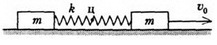
\includegraphics{051998CenterOfMassSpring.jpg}
\end{figure}

\AddProb Шар массой $m$ налетает со скоростью $v$ на покоящийся шар массой $2m$. 
Найдите скорости обоих шаров после упругого центрального удара. 

%6
\AddProb Определите, какую часть своей кинетической энергии теряет частица массой $m_1$ при упругом лобовом столкновении 
с неподвижной частицей массой $m_2$. 

\AddProb Известно, что при упругом нецентральном ударе двух одинаковых шаров, один из которых до удара покоился, 
угол разлета равен $90^{\circ}$. Докажите это утверждение.

\AddProb (2009) Невесомый стержень длины $L$ с двумя шариками на концах с массами $m$ и $3m$ находится на гладкой горизонтальной плоскости. 
Шарику массой $m$ резко сообщают скорость $v$ в направлении, перпендикулярном стержню. Какова сила натяжения стержня? 
Как изменится ответ, если скорость $v$ сообщить шарику массой $3m$? Какая часть энергии перейдет в кинетическую энергию вращательного движения в первом и втором случаях?

\AddProb (2012) На абсолютно гладком столе лежит обруч массой $M$ и радиусом $R$. На обруче находится жук, масса которого $m$. 
Какие траектории будут описывать жук и центр обруча при движении жука по обручу?

\begin{wrapfigure}{r}{5.5cm}
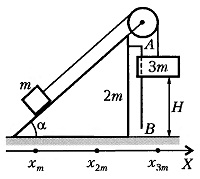
\includegraphics{0510CenterOfMassWedge.jpg}
\end{wrapfigure}

\AddProb Клин массой $2m$ с углом наклона к горизонту $\alpha $ ($\cos~\alpha$~=~2/3) находится на гладкой горизонтальной поверхности стола. 
Через блок, укрепленный на вершине клина, перекинута легкая нить, связывающая грузы массами $m$ и $3m$. 
Груз массой $3m$ может скользить вдоль вертикальной направляющей АВ, закрепленной на клине. 
Этот груз вначале удерживают неподвижно на расстоянии $H$~=~27~см от стола, а затем отпускают. 
На какое расстояние сместится клин к моменту касания груза массой $3m$ стола? Массами блока и направляющей АВ пренебречь.


\section{Распределенная масса}

%11
\AddProb Струя воды сечением $S$ ударяется о стенку, расположенную перпендикулярно струе. 
Скорость воды в струе $v$, после удара вода теряет скорость и стекает по стенке. Какова сила давления воды на стенку? Плотность воды $\rho$.

\AddProb Космический корабль массой $M$ движется в глубоком космосе. Для управления кораблем используется реактивный двигатель, 
который выбрасывает реактивную струю со скоростью $u$ относительно корабля, причем расход топлива в струе равен $\mu$ 
(расход топлива -- это масса топлива, выбрасываемая за единицу времени). Найдите ускорение корабля.

\begin{wrapfigure}{r}{2.5cm}
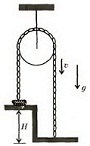
\includegraphics{0503DistributedMassChainAndPulley.jpg}
\end{wrapfigure}

\AddProb Длинная тонкая цепочка перекинута через блок так, что ее правая часть свисает до пола, а левая лежит, 
свернувшись клубком, на уступе высотой $H$. Цепочку отпускают, и она приходит в движение. 
Найдите установившуюся скорость движения цепочки. Блок идеальный, цепочка неупругая.

\AddProb Тонкое веревочное кольцо массой $m$ и радиусом $R$ положили на гладкую горизонтальную поверхность и 
раскрутили до угловой скорости $\omega$. Найдите силу натяжения веревки.

\begin{figure}[!h]
	\begin{subfigure}{.3\textwidth}
		\centering
		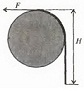
\includegraphics{0505DistributedMassRope.jpg}
	\end{subfigure}		
	\begin{subfigure}{.7\textwidth}
		\centering
		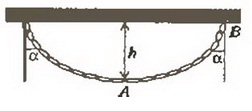
\includegraphics{0506DistributedMassChainAndCeiling.jpg}
	\end{subfigure}		
\end{figure}

\AddProb Веревку длиной $l$ и массой $m$ кладут на гладкое горизонтальное бревно радиусом $R$, 
причем вначале веревку удерживают за верхний конец, прикладывая горизонтальную силу $F$, а затем отпускают. 
Определите: 1) значение силы $F$; 2) ускорение веревки в первый момент.

%16
\AddProb Цепочку массой $m$ и длиной $l$ подвесили за концы к потолку. 
При этом оказалось, что в местах закрепления цепочка образует углы $\alpha $ с вертикалью. 
Найдите расстояние $h$ от нижней точки цепочки до потолка.

\begin{wrapfigure}{r}{3.5cm}
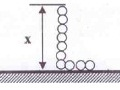
\includegraphics{0507DistributedMassChainAndTable.jpg}
\end{wrapfigure}

\AddProb (2011) Однородная цепочка длиной $L$ и массой $m$ подвешена на нити так, что другим концом она касается стола. 
Нить пережигают. Найти зависимость силы давления $F$ цепочки на стол от длины $x$ еще не упавшей части. Считать удар звеньев о стол неупругим.